%% Listas convertidas em prosa em 15/11/2026: 12 de 14. As duas mantidas sao
%% GLOSSARIOS DE NOTACAO imediatamente apos a definicao a que se referem (as
%% componentes da tupla do MDP e os termos da regra de atualizacao do Q). Isso e
%% convencao matematica, nao lista didatica: converter em prosa corrida piora a
%% consulta, que e a funcao delas.
%% Revisao estilistica em 15/11/2026. Reescritos a abertura e o paragrafo de
%% fechamento. O fecho anterior afirmava o "potencial do aprendizado por
%% reforco como componente fundamental" da proposta -- promessa da
%% qualificacao que a avaliacao nao sustenta. Ele agora declara o contrario,
%% que a camada principal arbitra por limiar deterministico, e diz por que.
\section{Aprendizado por Reforço}
\label{sec:fund-rl}

O Aprendizado por Reforço (\textit{Reinforcement Learning}, RL) aprende uma política por interação com o ambiente, sem exemplos rotulados de ação correta. Esta seção percorre seus elementos formais, os algoritmos relevantes para controle robótico e as razões pelas quais a camada principal desta tese não adota uma política aprendida. 

\subsection{Fundamentos do Aprendizado por Reforço}

O aprendizado por reforço é um paradigma onde um agente aprende a tomar decisões sequenciais através de interações com um ambiente, recebendo recompensas ou penalidades como feedback \cite{Sutton2018}. Diferentemente do aprendizado supervisionado ou não-supervisionado, o aprendizado por reforço foca na maximização de uma recompensa cumulativa ao longo do tempo \cite{Arulkumaran2017DeepRL}. A \autoref{fig:agente_ambiente} mostra o ciclo de interação entre o agente e o ambiente no aprendizado por reforço.

\begin{figure}[h]
    \centering
%% Figura refeita em 14/11/2026. A versao anterior omitia o ESTADO -- elemento central
%% do paradigma, listado logo abaixo e presente em toda a formalizacao do MDP -- e
%% trazia uma segunda seta do agente para o ambiente, horizontal e sem rotulo nenhum.
    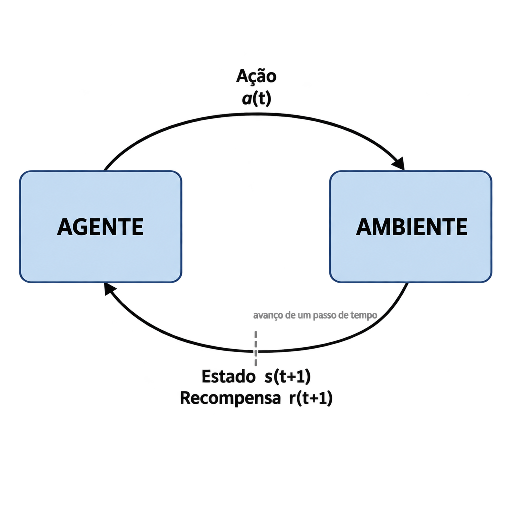
\includegraphics[width=0.8\textwidth]{figuras/fig_agente_ambiente.pdf}
    \caption{Ciclo de interação agente--ambiente no aprendizado por reforço. O agente
    emite a ação $a(t)$; o ambiente devolve o novo estado $s(t+1)$ e a recompensa
    $r(t+1)$, com o avanço de um passo de tempo assinalado sobre a seta de retorno.}
    \legend{Fonte: Elaborada pelo autor com base em \citeonline{Sutton2018}.}
    \label{fig:agente_ambiente}
\end{figure}


\subsubsection{Elementos Fundamentais}

O framework do aprendizado por reforço é composto por cinco elementos
\cite{Sutton2018}. O \emph{agente} é a entidade que decide e aprende, um robô autônomo
no caso que interessa aqui, e o \emph{ambiente} é o mundo com que ele interage, a
subestação. O \emph{estado} $s \in S$ representa a situação corrente de ambos; a
\emph{ação} $a \in A$ é a decisão do agente, capaz de alterar essa situação; e a
\emph{recompensa} $r \in \mathbb{R}$ é um escalar que informa o sucesso imediato da ação
executada. Toda a dificuldade do paradigma está nesse último elemento, porque um escalar
por passo é um canal estreito para comunicar o que se quer de um comportamento.

\subsubsection{Processo de Decisão de Markov}

O aprendizado por reforço é frequentemente formalizado como um Processo de Decisão de Markov (MDP), definido pela tupla $(S, A, P, R, \gamma)$ \cite{Puterman2014}:

\begin{itemize}
    \item $S$ é o conjunto de estados possíveis.
    \item $A$ é o conjunto de ações possíveis.
    \item $P: S \times A \times S \rightarrow [0, 1]$ é a função de transição de estados.
    \item $R: S \times A \times S \rightarrow \mathbb{R}$ é a função de recompensa.
    \item $\gamma \in [0, 1]$ é o fator de desconto, que determina a importância de recompensas futuras.
\end{itemize}

A propriedade de Markov estabelece que o próximo estado e a recompensa dependem apenas do estado atual e da ação tomada, não da história completa de estados e ações anteriores.

\subsubsection{Política e Função Valor}

O objetivo do agente é aprender uma política ótima $\pi^*: S \rightarrow A$ que maximize a recompensa cumulativa esperada. A política $\pi$ mapeia estados para ações (ou distribuições de probabilidade sobre ações) \cite{Sutton2018}.

A recompensa cumulativa descontada a partir do estado $s$ seguindo a política $\pi$ é definida como:

\begin{equation}
G_t = \sum_{k=0}^{\infty} \gamma^k R_{t+k+1}
\end{equation}

Duas funções são usadas para avaliar políticas. A \emph{função valor de estado}
$V^{\pi}$ dá o valor esperado de seguir a política $\pi$ a partir do estado $s$,

\begin{equation}
V^{\pi}(s) = \mathbb{E}_{\pi}[G_t | S_t = s]
\end{equation}

enquanto a \emph{função valor de ação} $Q^{\pi}$ dá o valor esperado de executar a ação
$a$ no estado $s$ e só então seguir $\pi$,

\begin{equation}
Q^{\pi}(s, a) = \mathbb{E}_{\pi}[G_t | S_t = s, A_t = a]
\end{equation}

distinção que importa porque é sobre a segunda, e não sobre a primeira, que se pode
decidir uma ação sem conhecer a dinâmica do ambiente.

\subsection{Algoritmo Q-Learning e Variantes}

O Q-Learning é um dos algoritmos mais fundamentais e amplamente utilizados no aprendizado por reforço, especialmente em aplicações robóticas \cite{Watkins1992}.

\subsubsection{Q-Learning Clássico}

O Q-Learning é um algoritmo livre de modelo (\textit{model-free}) que aprende diretamente a função valor ótima $Q^*$ sem necessidade de conhecer a dinâmica do ambiente \cite{Watkins1992}.

O algoritmo atualiza iterativamente a estimativa da função $Q$ usando a seguinte regra:

\begin{equation}
Q(s_t, a_t) \leftarrow Q(s_t, a_t) + \alpha [r_{t+1} + \gamma \max_{a} Q(s_{t+1}, a) - Q(s_t, a_t)]
\label{eq:fund-qlearning}
\end{equation}

Onde:
\begin{itemize}
    \item $\alpha \in (0, 1]$ é a taxa de aprendizado.
    \item $r_{t+1}$ é a recompensa recebida após executar a ação $a_t$ no estado $s_t$.
    \item $\gamma$ é o fator de desconto.
    \item $\max_{a} Q(s_{t+1}, a)$ é o valor máximo estimado para o próximo estado $s_{t+1}$.
\end{itemize}

%% Acrescentado em 15/11/2026. O capitulo ensinava a regra de atualizacao sem nomear a
%% equacao de Bellman, e a Secao 4.6 fala da "equacao de Bellman" e rotula sua equacao
%% como eq:prop-bellman. "Bellman" ocorria ZERO vezes em todo o Capitulo 2 e 3 vezes
%% nos capitulos posteriores: o leitor encontrava o nome depois do uso.
A expressão entre colchetes na Equação~\eqref{eq:fund-qlearning} é o \emph{erro de
diferença temporal}: a discrepância entre o valor estimado para o par corrente e a
estimativa revista à luz da recompensa observada e do melhor valor disponível no estado
seguinte. A regra desloca a estimativa na direção dessa discrepância, numa fração
$\alpha$ dela. O ponto fixo dessa iteração é a \emph{equação de Bellman} de otimalidade,
\begin{equation}
Q^*(s,a) = \mathbb{E}\!\left[\, r + \gamma \max_{a'} Q^*(s',a') \,\right],
\label{eq:fund-bellman}
\end{equation}
que caracteriza a função valor ótima por uma condição de consistência: o valor de um par
estado-ação é a recompensa imediata esperada mais o valor descontado do melhor que se pode
fazer em seguida. Não é uma regra de cálculo, e sim a identidade que a solução satisfaz; o
Q-Learning é um dos procedimentos que convergem para ela. Essa distinção entre a
\emph{identidade} e o \emph{procedimento} será retomada no
Capítulo~\ref{cap:proposta}, onde se discute o que significa acrescentar um termo à
atualização sem alterar a identidade que ela persegue.

Uma característica importante do Q-Learning é o dilema exploração-explotação: o agente precisa balancear entre explorar novas ações (para descobrir melhores estratégias) e explotar o conhecimento atual (para maximizar recompensas). A estratégia $\epsilon$-greedy é comumente utilizada, onde com probabilidade $\epsilon$, escolhe-se uma ação aleatória (exploração); caso contrário, escolhe-se a ação com maior valor Q (explotação).

\subsubsection{Variantes do Q-Learning}

\paragraph{SARSA}

SARSA (State-Action-Reward-State-Action) é uma variante do Q-Learning que utiliza a política atual para atualizar os valores Q \cite{Rummery1994}. A regra de atualização é:

\begin{equation}
Q(s_t, a_t) \leftarrow Q(s_t, a_t) + \alpha [r_{t+1} + \gamma Q(s_{t+1}, a_{t+1}) - Q(s_t, a_t)]
\end{equation}

A principal diferença entre Q-Learning e SARSA é que o Q-Learning é um algoritmo \textit{off-policy} (aprende a política ótima independentemente da política de exploração), enquanto SARSA é \textit{on-policy} (aprende a política que está sendo seguida).

\paragraph{Double Q-Learning}

O Double Q-Learning foi proposto para mitigar o problema de superestimação presente no Q-Learning tradicional \cite{Hasselt2010}. O algoritmo mantém duas funções valor, $Q_A$ e $Q_B$, e utiliza uma para selecionar ações e outra para avaliá-las, reduzindo o viés de superestimação.

%% Secao COMPRIMIDA e ACRESCIDA em 15/11/2026. Antes: 317 palavras sobre DQN e
%% algoritmos de politica, com figura propria, e NADA sobre moldagem de recompensa.
%% O desequilibrio era mensuravel: "DQN" ocorria 6 vezes aqui e zero nos Capitulos 4
%% a 7, enquanto `shaping' e `invariancia de politica' ocorriam ZERO aqui e 3 vezes na
%% Secao 4.7, onde esta tese declara que seu campo NAO tem a forma potencial de Ng. O
%% leitor precisava ja saber o que e essa garantia para entender o que estava sendo
%% renunciado. O DQN foi mantido em forma curta porque o Capitulo 3 depende dele (13
%% ocorrencias de DRL/DQN la), mas a figura fig_dqn saiu: ela detalhava rede alvo e
%% buffer de repeticao, que nenhum capitulo posterior usa.
\subsection{Aprendizado por Reforço Profundo}

O aprendizado por reforço profundo substitui a tabela de valor por um aproximador
paramétrico, o que o torna aplicável a espaços de estado de alta dimensão onde a tabela
seria intratável \cite{Arulkumaran2017DeepRL}. A \textit{Deep Q-Network} aprende
$Q(s,a;\theta)$ com uma rede neural em lugar de uma entrada por par estado-ação
\cite{Mnih2015}, e as duas técnicas que a tornaram treinável atacam a mesma dificuldade,
a correlação entre amostras consecutivas: a repetição de experiências treina a rede com
mini-lotes sorteados de um \textit{buffer} de transições, quebrando a ordem temporal, e a
rede alvo mantém uma segunda cópia de parâmetros atualizada apenas periodicamente, de
sorte que o alvo da regressão não se desloca a cada passo junto com a rede que o persegue.
Uma segunda família aprende a política diretamente, em vez de derivá-la de uma função
valor \cite{Sutton1999}: os métodos \textit{actor-critic} acoplam um aprendiz de política
a um de valor \cite{Konda1999}, e o \ac{PPO} limita a magnitude de cada atualização para
estabilizar o treino \cite{Schulman2017}. Nenhuma dessas famílias é empregada nesta tese,
que opera com tabela de valor discreta; elas aparecem aqui porque a literatura revisada no
Capítulo~\ref{cap:revisao} é majoritariamente construída sobre elas.

\subsection{Moldagem de Recompensa e Invariância de Política}
\label{sec:fund-shaping}

Recompensa esparsa torna o aprendizado lento: se o sinal só chega ao alcançar o objetivo,
o agente precisa encontrá-lo por exploração antes de ter o que aprender. A \emph{moldagem
de recompensa} acrescenta à recompensa original $r$ um termo $F$ que oferece sinal
intermediário, de modo que o agente aprende sobre a soma $r+F$ em vez de sobre $r$. O
expediente é antigo e eficaz, mas introduz um risco que lhe é próprio: um termo mal
escolhido pode deslocar a política ótima, premiando um comportamento que acumula $F$ sem
cumprir a tarefa --- o caso extremo é o agente que circula indefinidamente entre estados
de alto $F$ em vez de terminar.

\citeonline{ng1999} delimitaram exatamente quando esse risco não existe. O resultado é que
$F$ preserva a política ótima para \emph{qualquer} recompensa original se e somente se
tiver a forma \emph{potencial}
\begin{equation}
F(s,a,s') = \gamma\,\Phi(s') - \Phi(s),
\label{eq:fund-shaping}
\end{equation}
isto é, se for a diferença descontada de uma função $\Phi$ sobre estados. A propriedade
tem nome: \emph{invariância de política} sob transformação de recompensa. A intuição é que
um termo dessa forma se cancela ao longo de qualquer trajetória fechada, de sorte que
nenhum ciclo acumula recompensa artificial, e o que ele altera é a velocidade do
aprendizado, não o seu destino.

A distinção importa porque fixa o ônus da prova. Um termo aditivo que \emph{não} assuma a
forma da Equação~\eqref{eq:fund-shaping} --- por ser variante no tempo, por depender de
evento observado ou por somar-se diretamente ao valor em vez de entrar como diferença de
potencial --- não herda garantia alguma, e qualquer afirmação sobre a política resultante
precisa ser demonstrada caso a caso. A Seção~\ref{sec:prop-atualizacao} retoma esse
ponto para declarar o estatuto do campo formulado nesta tese, que é precisamente um termo
dessa segunda espécie.
\subsection{Aplicações em Robótica Autônoma}

O aprendizado por reforço tem sido aplicado em robótica autônoma sobretudo em percepção, navegação e manipulação \cite{Kober2013}.

\subsubsection{Navegação Autônoma}

A navegação autônoma é uma das aplicações mais relevantes do aprendizado por reforço em robótica, especialmente em ambientes dinâmicos e não estruturados como subestações elétricas \cite{Faria2002}.

Para um robô móvel, o problema de navegação pode ser formulado como um MDP em que os
estados são representações da posição, da orientação e da percepção sensorial do robô, as
ações são comandos de movimento, tipicamente velocidades linear e angular, e as
recompensas são positivas na aproximação ao objetivo e negativas em colisões e em
comportamentos indesejados. É na terceira dessas escolhas que se concentra o trabalho de
projeto, porque ela precisa codificar, num escalar, tudo o que distingue uma trajetória
aceitável de uma inaceitável.

As abordagens de aprendizado por reforço aplicadas à navegação robótica distinguem-se
pelo que supõem sobre o mapa. A navegação \emph{baseada em mapas} aprende a se deslocar
sobre uma representação do ambiente, frequentemente combinando aprendizado com técnicas
de SLAM. A navegação \emph{reativa} dispensa o mapa explícito e aprende a responder
diretamente às percepções sensoriais \cite{Zhu2017,Tai2017}.
%% Corrigido em 14/11/2026 (auditoria bibliografica): Tai2017 sustentava o item de
%% navegacao baseada em mapas, mas o proprio titulo do trabalho e "continuous control
%% of mobile robots for MAPLESS navigation" -- e a categoria oposta. A citacao foi
%% retirada daquele item (a categoria e descritiva e nao precisa de apoio pontual) e
%% passada ao item reativo, onde descreve corretamente a fonte.
A navegação \emph{hierárquica} combina as duas, com planejamento de alto nível sobre
controle reativo de baixo nível \cite{Kulkarni2016}, e é a essa terceira família que a
arquitetura desta tese se filia, com a diferença de que a camada de alto nível aqui não
é aprendida.

\subsubsection{Inspeção Autônoma}

%% Reescrito em 13/11/2026 (auditoria bibliografica): a referencia anterior desta
%% frase nao foi localizada em nenhuma base. A alegacao de aplicacao bem-sucedida de
%% aprendizado por reforco a inspecao de subestacoes foi retirada; o que a literatura
%% verificada sustenta e o uso de aprendizado em navegacao sobre observacoes fundidas,
%% em robotica movel, e nao em inspecao de subestacao em operacao.
O aprendizado por reforço tem sido aplicado a tarefas de navegação autônoma sobre observações sensoriais fundidas \cite{Ou2024SensorFusionDRL}; sua transposição para a inspeção de infraestruturas críticas como subestações elétricas permanece, em larga medida, uma direção em aberto.

Em aplicações de inspeção, o aprendizado por reforço pode ser empregado no planejamento
de trajetórias que maximizem cobertura e qualidade, na detecção e investigação de
anomalias encontradas durante a ronda, e na adaptação do comportamento a condições
ambientais variáveis. As três tarefas diferem em horizonte: a primeira é decidida antes
da missão, a segunda durante, e a terceira ao longo de missões sucessivas.

\subsection{Desafios e Limitações}

%% Reescrito em 15/11/2026. A frase abria por "Apesar de seu potencial" e terminava em
%% dois-pontos, mas o que vinha depois era um \subsubsection: os dois-pontos nao
%% anunciavam nada. As tres restricoes nomeadas sao exatamente as tres subsecoes.
A transposição do aprendizado por reforço de jogos e de ambientes de teste simulados para o robô físico esbarra em três restrições operacionais \cite{Kober2013, Arulkumaran2017DeepRL}, tratadas nas três subseções seguintes.

\subsubsection{Eficiência de Amostra}

O aprendizado por reforço frequentemente requer um grande número de interações com o
ambiente para aprender políticas eficazes, o que é impraticável em robótica real pelo
tempo e pelo desgaste envolvidos. As mitigações usuais deslocam o custo em vez de
removê-lo: treinar em simulação antes de transferir para o mundo real troca interações
reais por uma lacuna de domínio a vencer; inicializar a política com demonstrações
humanas ou de outro sistema troca-as pela qualidade do que se demonstrou; e reutilizar
conhecimento de tarefas anteriores troca-as pela semelhança entre as tarefas, que precisa
ser verdadeira.

\subsubsection{Exploração Segura}

Em robótica, a exploração aleatória pode levar a comportamentos que danificam o robô ou o
ambiente, e os métodos de exploração segura diferem em onde colocam a restrição. A
exploração guiada por incerteza a coloca na escolha da próxima ação, dirigindo-a para
onde o agente sabe menos. As restrições de segurança a colocam na formulação do problema
ou na função de recompensa, antes do aprendizado. E as formulações com risco limitado a
colocam no critério otimizado, que passa a penalizar explicitamente a cauda ruim em vez
da média. Nesta tese a restrição está em outro lugar ainda: fora da política, numa regra
de precedência que o aprendizado não pode negociar.

\subsubsection{Generalização e Transferência}

Políticas aprendidas em um ambiente ou configuração específica frequentemente não
generalizam para novos, e os três obstáculos reconhecidos são de naturezas distintas. A
transferência \textit{sim-to-real} enfrenta uma diferença sistemática entre o simulador e
o mundo. A adaptação a ambientes não vistos no treinamento enfrenta uma diferença entre
instâncias do mesmo tipo de ambiente. E a robustez a perturbações enfrenta variação
dentro de uma única instância, durante a operação. Confundir as três faz um resultado de
simulação parecer uma garantia de campo.

\subsection{Integração com Outros Paradigmas}

Para superar as limitações do aprendizado por reforço puro, abordagens híbridas que integram outros paradigmas têm sido propostas \cite{Kober2013}:

\subsubsection{Integração com Controle Clássico}

A combinação de aprendizado por reforço com controle clássico admite três arranjos, que
diferem em qual dos dois tem a palavra final. Modelos aprendidos podem alimentar
controladores clássicos, melhorando-lhes a predição sem alterar a estrutura de controle.
Controladores clássicos podem guiar a exploração durante o aprendizado, restringindo o
que o agente chega a experimentar. E arquiteturas híbridas podem reservar as tarefas
críticas de segurança ao controlador clássico e deixar à política aprendida apenas a
otimização de desempenho, que é a divisão de responsabilidade mais próxima da adotada no
Capítulo~\ref{cap:proposta}.

\subsubsection{Integração com Planejamento Simbólico}

A integração de aprendizado por reforço com planejamento simbólico atende a tarefas de
longo prazo por três vias. Hierarquias de abstração reservam o alto nível ao planejamento
simbólico e a execução ao aprendizado. Representações simbólicas facilitam transferir
conhecimento entre tarefas, porque descrevem a tarefa em termos que sobrevivem à troca de
ambiente. E conhecimento causal explícito melhora a eficiência do aprendizado e a
interpretabilidade da política resultante, que é precisamente o que falta às políticas
puramente aprendidas quando se exige certificação.

\subsection{Aplicações Específicas em Subestações Elétricas}

A literatura aponta quatro usos do aprendizado por reforço na inspeção autônoma de
subestações \cite{Ou2024SensorFusionDRL, Wei2024Advancements}: aprender políticas de
navegação que se adaptem à interferência eletromagnética variável; aprender a priorizar
equipamentos por criticidade, histórico de falhas e indicadores de anomalia; aprender a
investigar a anomalia detectada, ajustando o comportamento para coletar informação
adicional quando necessário; e ajustar a estratégia de inspeção a condições de
iluminação, clima e interferência. Os quatro supõem que a decisão a ser aprendida seja a
decisão de inspeção, e é exatamente essa suposição que esta tese não adota.

A camada principal desta tese não usa política aprendida. O arbítrio entre inspecionar e se afastar é resolvido por limiar determinístico (Capítulo~\ref{cap:proposta}), escolha que decorre de duas das limitações expostas acima, a eficiência de amostra e a opacidade da política treinada; a tabela \textit{Q} comparece no trabalho como linha de base comparativa (Seção~\ref{sec:setup-qdriven}).
